\chapter{PHƯƠNG PHÁP NGHIÊN CỨU}
\label{chap:Chapter3}

Bản chất của các phương pháp dựa trên neural network là ước lượng xác suất của dữ liệu (probability density) nên cần chuẩn hóa (normalization), trong khi mô hình Diffusion sẽ học để có thể ước lượng đạo hàm của phân phối dữ liệu \cite{song2021score} (estimating gradients of data distribution) và không phải chuẩn hóa trên toàn bộ dữ liệu, nên có kết quả tốt hơn so với các phương pháp neural network không sử dụng diffusion. Mô hình diffusion có khả năng mô phỏng phân phối dữ liệu trong các trường hợp mật độ phân phối của dữ liệu thấp và có thể sinh được kết quả với độ chi tiết cao.

Mô hình của luận văn dựa trên mô hình DiffuseStyleGesture \cite{yang2022DiffuseStyleGestureplus} với cải tiến chính là dựa trên dữ liệu giọng nói, luận văn chuyển giọng nói thành văn bản và nhúng văn bản để thu được các vector đặc trưng văn bản, và sử dụng như là một vector đặc trưng về ngữ nghĩa trong quá trình diffusion có điều kiện. Quá trình này được trình bày \autoref{subsec:feature_extraction}. Ngoài ra ở công đoạn \textit{7. Kết xuất}  (\autoref{fig:CommonStage}), luận văn sử dụng Unity để trực quan hoá kết quả sinh cử chỉ.
Các đóng góp chính của luận văn được trình bày đầy đủ ở \autoref{sec:contribution}.

Trước tiên luận văn trình bày về mô hình diffusion \autoref{sec:summary_diffusion}, và phần \autoref{sec:ohgesture} sẽ trình bày về mô hình đề xuất OHGesture.

\section{Mô hình diffusion cơ bản và các cải tiến}
\label{sec:summary_diffusion}

\begin{figure}[H]
	\centering
	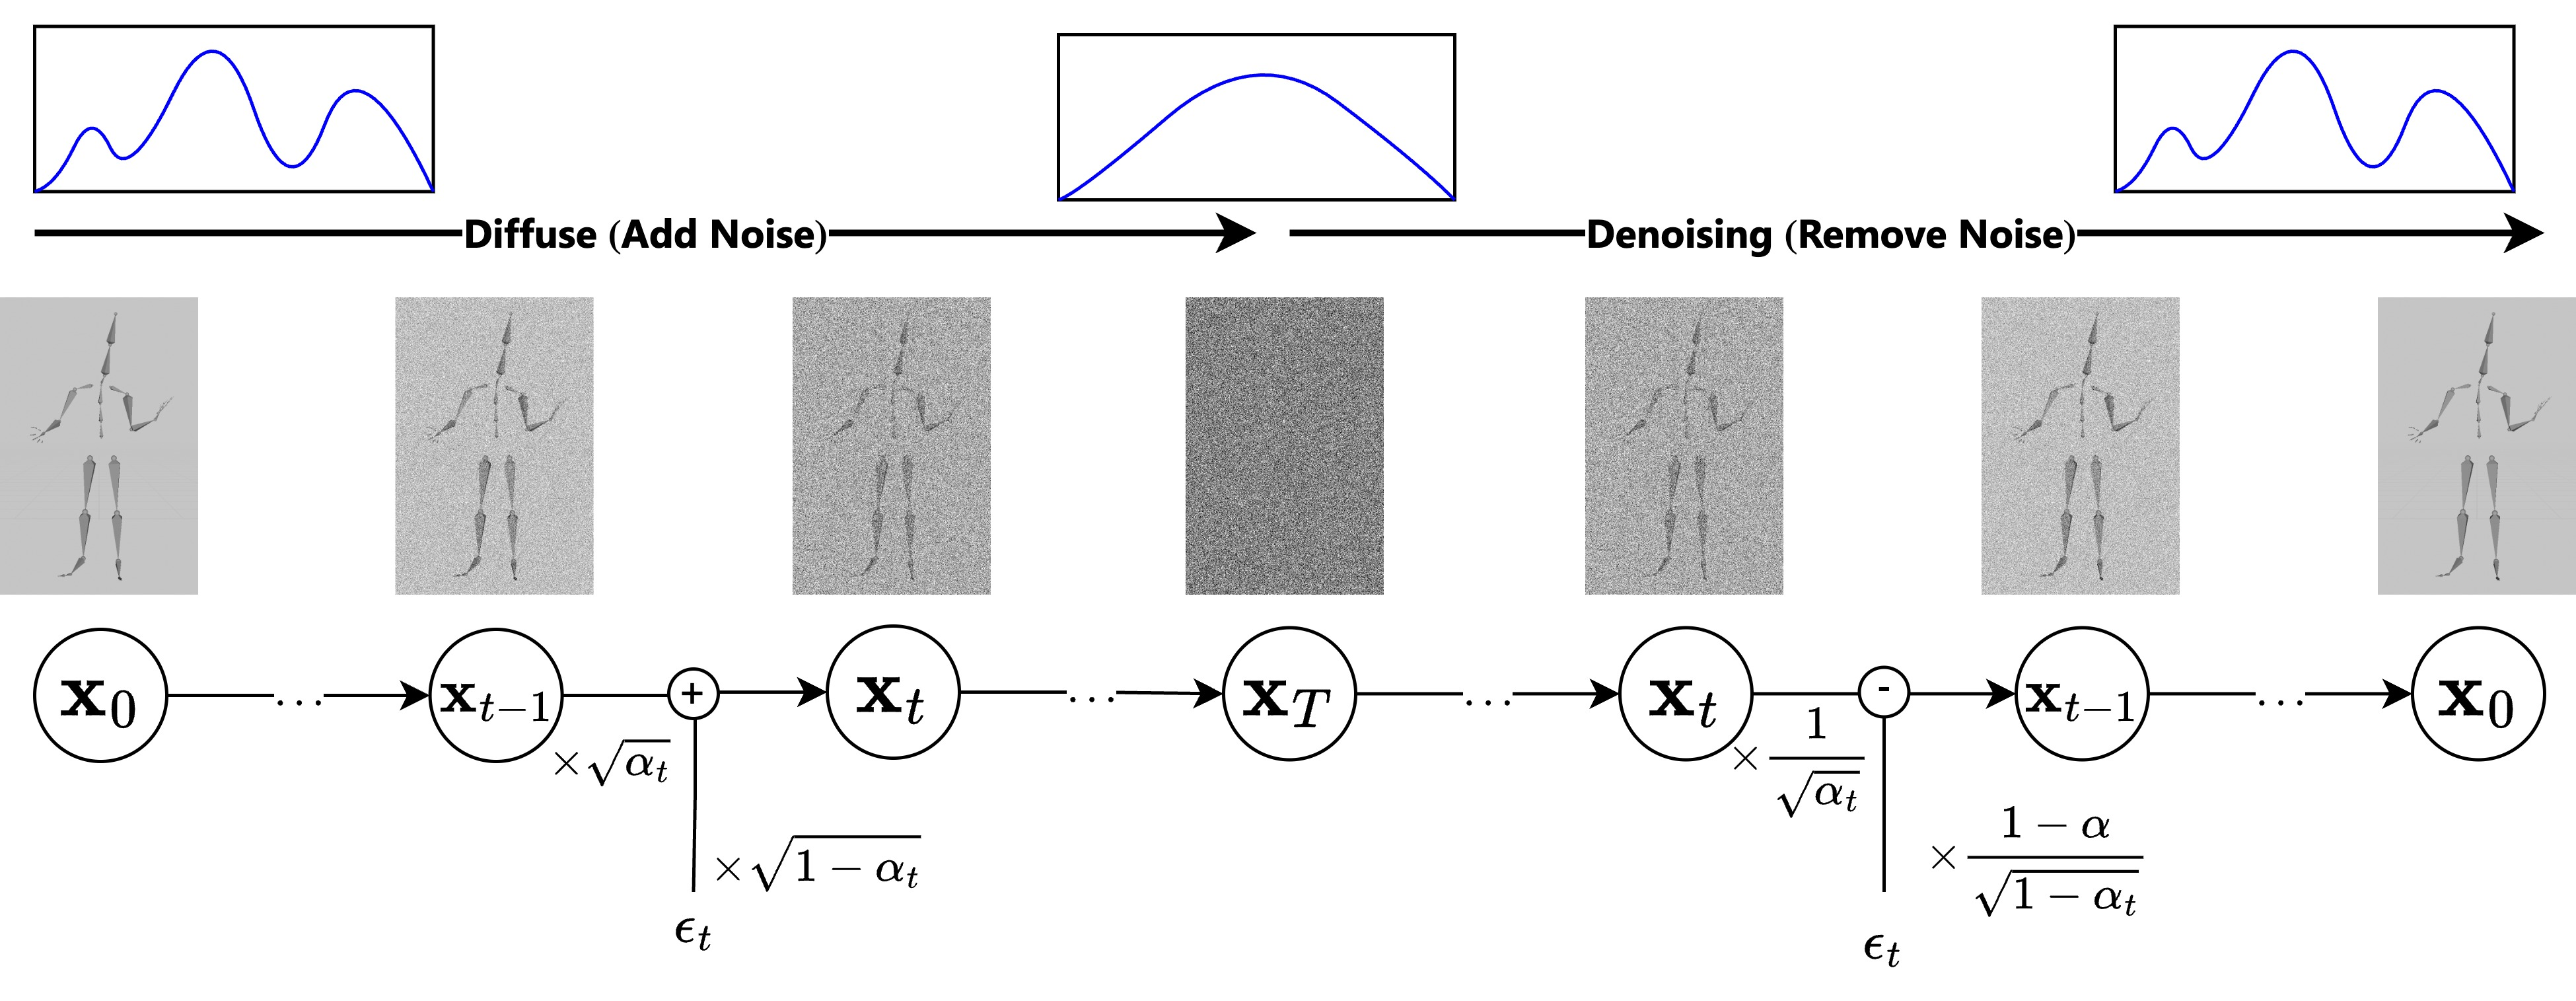
\includegraphics[width=\linewidth]{DiffuseAndDenoise}
	\caption{Quá trình gây nhiễu (Diffuse) và khử nhiễu (Denoise) \textbf{không} huấn luyện}
	\label{fig:DiffuseAndDenoise}
\end{figure}

Với các phương pháp sử dụng neural network như ResNet, InceptionNet,... kết quả là tìm được trọng số $\theta$ của hàm $f_{\theta}(x)$, mục tiêu là tối ưu hóa hàm lỗi $\mathcal{L}_\text{loss}$ giữa nhãn $y$ và kết quả dự đoán là $\hat{y}$. Sau khi kết thúc quá trình huấn luyện và học được trọng số $\theta'$ ta dự đoán một mẫu dữ liệu mới $x'$ bằng cách truyền qua hàm $f_{\theta'}$ để ra được kết quả dự đoán $y'$.

Tương tự phương pháp VAE, mã hóa (encode) ma trận đầu vào thành vector tiềm ẩn $z$ và giải mã (decode) vector tiềm ẩn $z$ trở lại ma trận kích thước ban đầu, tuy nhiên mô hình diffusion chia quá trình học thành từng $T$ bước, ở bước thứ $t$ quá trình gây nhiễu (forward diffusion process) $q(\mathbf{x})$ từ $1 \to T$ được thực hiện bằng cách thêm nhiễu $\epsilon_{t} \sim \mathcal{N} (\mathbf{0}, \mathbf{I})$ phân phối chuẩn Gaussian vào dữ liệu, với $\mathbf{I}$ là ma trận đơn vị của phân phối chuẩn Gaussian có giá trị trung bình  (mean) bằng $\mathbb{E}[\epsilon]=0$ và phương sai $\operatorname{Var}(\epsilon)=1$.


Quá trình thêm nhiễu từ trái qua phải gọi là hàm $q(\bx)$, còn quá trình khử nhiễu từ phải qua trái $p(\bx)$. Lưu ý rằng, $\epsilon_t$ được lấy ngẫu nhiên ở mọi bước $t$, và nhiễu $\epsilon_t$ được giữ cố định. Như trong \autoref{fig:DiffuseAndDenoise}, nếu ở bước thêm nhiễu (diffuse) ta \textbf{cộng} một lượng nhiễu $\epsilon_t$ và ở bước khử nhiễu (denoise) ta cũng \textbf{trừ} một lượng chính xác lượng nhiễu $\epsilon_t$ thì kết quả cuối cùng của bước khử nhiễu $\bx_0$ là \textbf{hoàn toàn giống} ảnh gốc ban đầu.

Tuy nhiên, ở bước khử nhiễu, thay vì \textit{trừ} đi nhiễu thực tế $\epsilon_t$ đã được thêm vào ở bước gây nhiễu, luận văn sẽ dùng một hàm $f_{\theta}$ để dự đoán \textbf{nhiễu được thêm vào} ở quá trình diffuse, từ đó lần lượt lấy ảnh nhiễu $\bx_T$ trừ đi nhiễu dự đoán để được ảnh dự đoán $\hat{\bx}_{T-1}$, thực hiện lần lượt cho đến khi đạt được $\hat{\bx}_0$.

Trong mô hình Diffusion cơ bản hay Denoising Diffusion Probabilistic Models (DDPM \cite{ho2020denoising}), quá trình khử nhiễu (denoising process) từ $T \to 1$, mục tiêu là học được trọng số $\theta$ của hàm dự đoán nhiễu $f_{\theta}$ hay còn được ký hiệu là hàm dự đoán lượng nhiễu ($\epsilon_\theta$) đã được thêm vào. Sau khi kết thúc quá trình học và thu được trọng số $\theta'$ của hàm dự đoán nhiễu $\hat{\epsilon}$, luận văn sẽ dùng hàm $f_{\theta'}$ để dự đoán nhiễu. Sau khi có nhiễu dự đoán $\hat{\epsilon}$, chúng ta trừ đi ảnh bị nhiễu $\mathbf{x}_{t}$ để có được ảnh khử nhiễu $\mathbf{x}_{t-1}$, và cộng thêm nhiễu $ \mathbf{z} \in \mathcal{N}(0, \mathbf{I})$ để tạo ra sự đa dạng cử chỉ. Thực hiện lần lượt từ $T \to 1$ để có được ảnh dự đoán $\hat{\bx_0}$.

\subsection{Quá trình gây nhiễu (forward diffusion process)}

Cho dữ liệu $\mathbf{x}_{0}$ được lấy từ dữ liệu thật $\mathbf{x}_{0} \sim q(x)$, với mỗi bước ta sẽ thêm nhiễu vào đầu vào $\bx_{0}$ với tỷ lệ giữa nhiễu và ảnh gốc được kiểm soát bằng hệ số $\beta$:


\begin{equation}
	\label{eq:addgaussian}
	\mathbf{x}_t = \sqrt{1 - \beta_t}\mathbf{x}_{t-1} + \sqrt{\beta_t} \boldsymbol{\epsilon}_{t-1}
\end{equation}


Trong đó, quá trình gây nhiễu từ $1 \to T$, với mỗi bước $t$, quá trình thêm nhiễu $\epsilon$ được điều khiển bởi $\beta_t$ thuộc tập hợp $\{\beta_t \in (0, 1)\}_{t=1}^T$.

Bởi vì một hàm $f(x)$ có dạng $f(x) = a x + b\epsilon$ với $\epsilon \in \mathcal{N}(0, \mathbf{I})$ sẽ tương đương $f(x) \sim \mathcal{N}(a x, b^2)$ (với $a x$ là kỳ vọng hay trung bình, $b^2$ là phương sai), từ đó quá trình gây nhiễu có thể được viết gọn là ở từng bước nhiễu $t$, khi biết trước $\bx_{t-1}$ là:

\begin{equation}
	\label{eq:forward_diffusion_process}
	\begin{aligned}
		q(\mathbf{x}_t \vert \mathbf{x}_{t-1}) &= \mathcal{N}(\mathbf{x}_t; \sqrt{1 - \beta_t} \mathbf{x}_{t-1}, \beta_t\mathbf{I}) \quad \\
		q(\mathbf{x}_{1:T} \vert \mathbf{x}_0) &= \prod^T_{t=1} q(\mathbf{x}_t \vert \mathbf{x}_{t-1})
	\end{aligned}
\end{equation}

Mục tiêu ở bước $t$ của hệ số $\sqrt{1 - \beta_t}$ và $\beta_t$ là để lần lượt giảm tỷ lệ của ảnh gốc $\mathbf{x}_t$ và tăng dần nhiễu  $\boldsymbol{\epsilon}_{t-1}$, vì vậy $\beta_1 < \beta_2 < \dots < \beta_T$. Khi $T \to \infty$ thì $\mathbf{x}_{T}$ sẽ nhiễu hoàn toàn \cite{weng2021diffusion} (Isotropic Gaussian Distribution) $q(\mathbf{x}_{T}) = \mathcal{N} (0, \mathbf{I})$.

\begin{figure}[H]
	\centering
	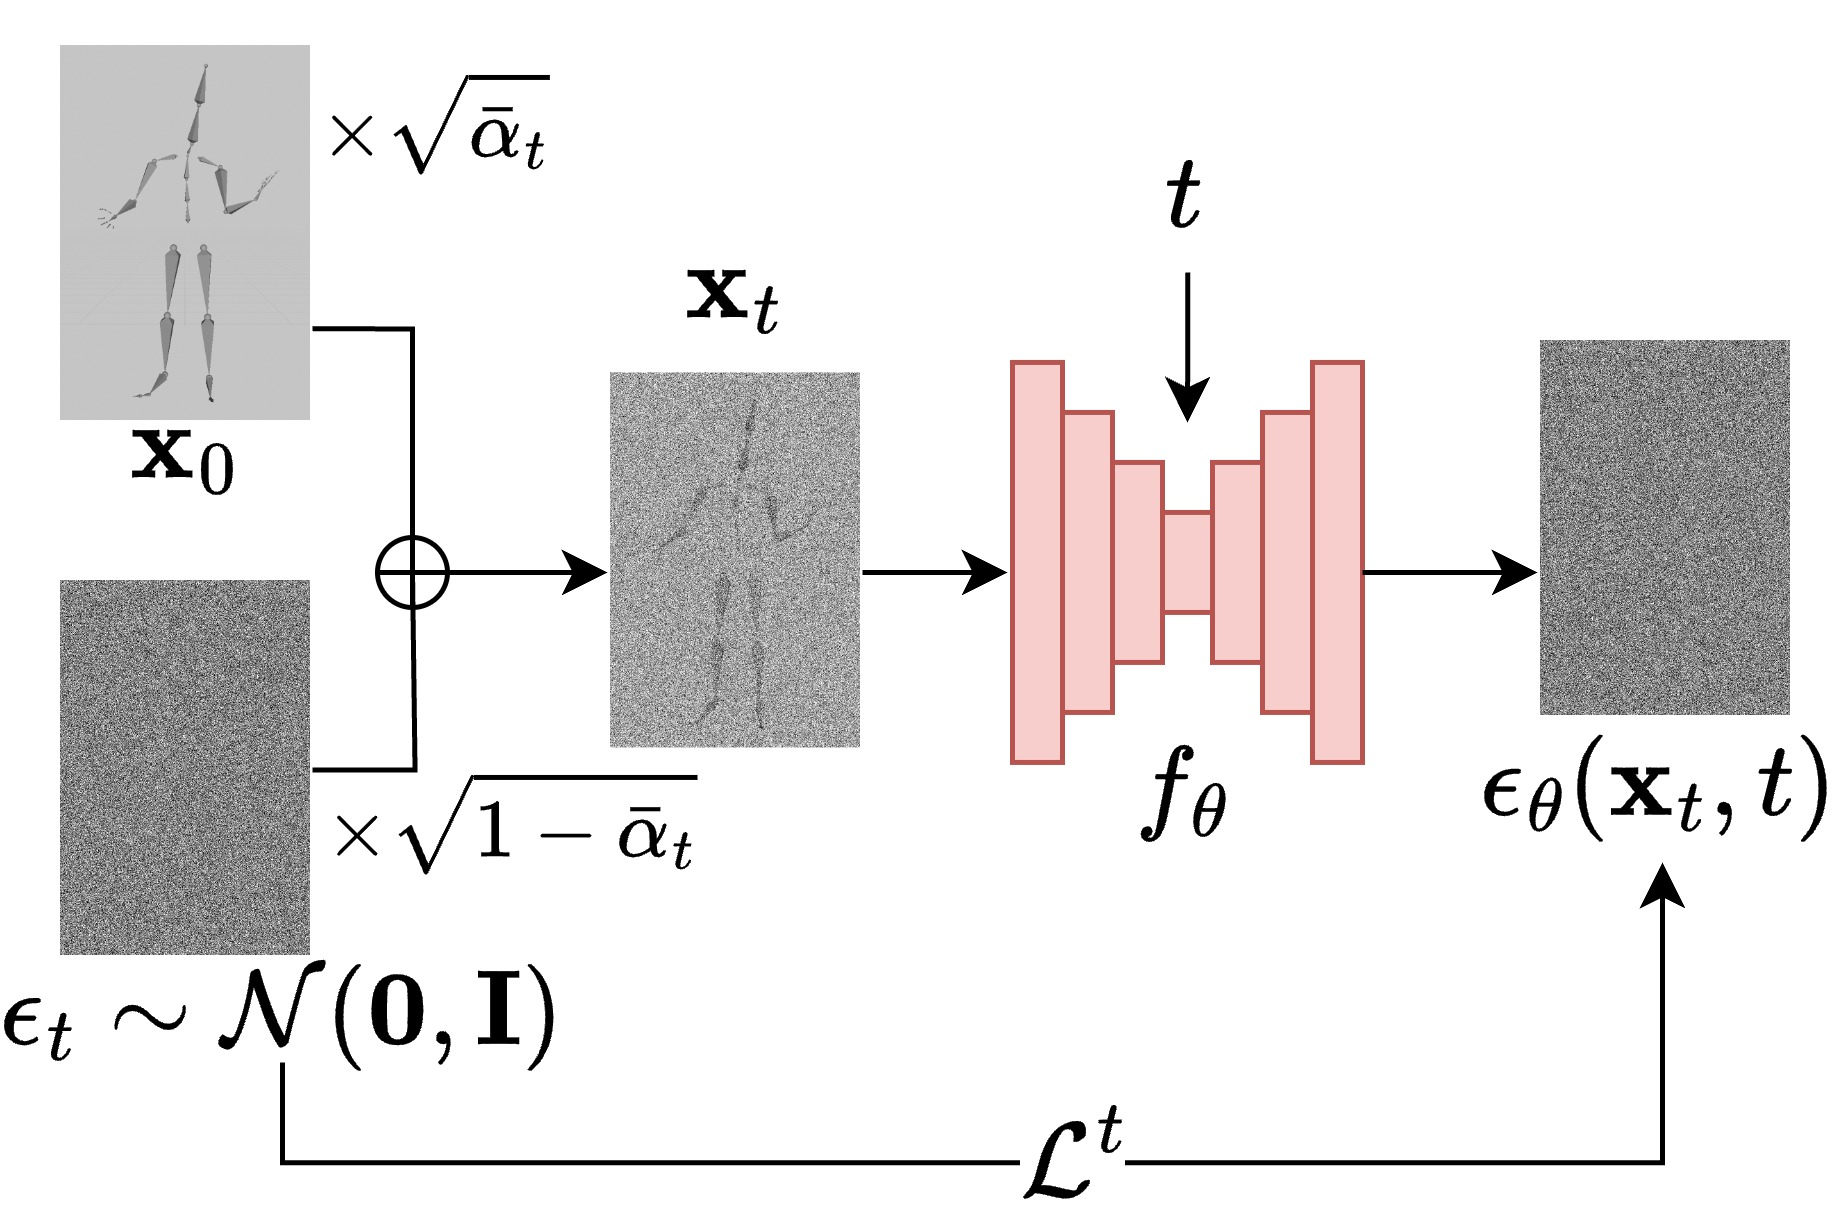
\includegraphics[height=160pt]{AlgorithmForwardDiffusion}
	\caption{Thêm nhiễu trong quá trình huấn luyện}
	\label{fig:AlgorithmForwardDiffusion}
\end{figure}

Vì nhiễu $\boldsymbol{\epsilon}_{t-1}, \boldsymbol{\epsilon}_{t-2}, \dots \sim \mathcal{N}(\mathbf{0}, \mathbf{I})$ luôn là các biến ngẫu nhiên tuân theo phân phối chuẩn Gaussian, và được xác định trước ở mỗi bước $t$, nên ta có thể dễ dàng tính $\bx_t$ từ $\bx_0$. Bằng cách đặt $\alpha_t = 1 - \beta_t$ và $\bar{\alpha}_t = \prod_{i=1}^t \alpha_i$, từ \autoref{eq:addgaussian}, ta có hàm forward diffusion viết lại theo $\alpha$ như sau:

\begin{equation}
\begin{aligned}
	\boldsymbol{x}_t &= \sqrt{\alpha_t}\boldsymbol{x}_{t-1} + \sqrt{1 - \alpha_t}\boldsymbol{\epsilon}_{t-1} \\
	&= \sqrt{\alpha_t}\left(\sqrt{\alpha_{t-1}}\boldsymbol{x}_{t-2} + \sqrt{1 - \alpha_{t-1}}\boldsymbol{\epsilon}_{t-2}\right) + \sqrt{1 - \alpha_t}\boldsymbol{\epsilon}_{t-1} \\
	&= \sqrt{\alpha_t\alpha_{t-1}}\boldsymbol{x}_{t-2} + \sqrt{\alpha_t(1 - \alpha_{t-1})}\boldsymbol{\epsilon}_{t-2} + \sqrt{1 - \alpha_t}\boldsymbol{\epsilon}_{t-1} \\
	&= \sqrt{\alpha_t\alpha_{t-1}}\boldsymbol{x}_{t-2} + \sqrt{\alpha_t(1 - \alpha_{t-1}) + (1 - \alpha_t)}\boldsymbol{\epsilon}_{t-2} \\
	&= \sqrt{\alpha_t\alpha_{t-1}}\boldsymbol{x}_{t-2} + \sqrt{1 - \alpha_t\alpha_{t-1}}\boldsymbol{\epsilon}_{t-2} \\
	&= \ldots \\
	&= \sqrt{\prod_{i=1}^t \alpha_i} \boldsymbol{x}_0 + \sqrt{1 - \prod_{i=1}^t \alpha_i} \boldsymbol{\epsilon}_0 \\
	&= \sqrt{\bar{\alpha}_t} \boldsymbol{x}_0 + \sqrt{1 - \bar{\alpha}_t} \boldsymbol{\epsilon}_0 \\
	&\sim \mathcal{N}\left(\boldsymbol{x}_t; \sqrt{\bar{\alpha}_t} \boldsymbol{x}_0, \left(1 - \bar{\alpha}_t\right) \textbf{I}\right)
\end{aligned}
\label{eq:tracexzero}
\end{equation}

Sự thay đổi của $\sqrt{\alpha}$ và  $\sqrt{1- \alpha}$ trong quá trình gây nhiễu được thể hiện ở phụ lục \autoref{appendix:Appendix1}

\subsection{Quá trình khử nhiễu (denoising process)}
\label{subsection:denoising_process}

\begin{figure}[H]
	\centering
	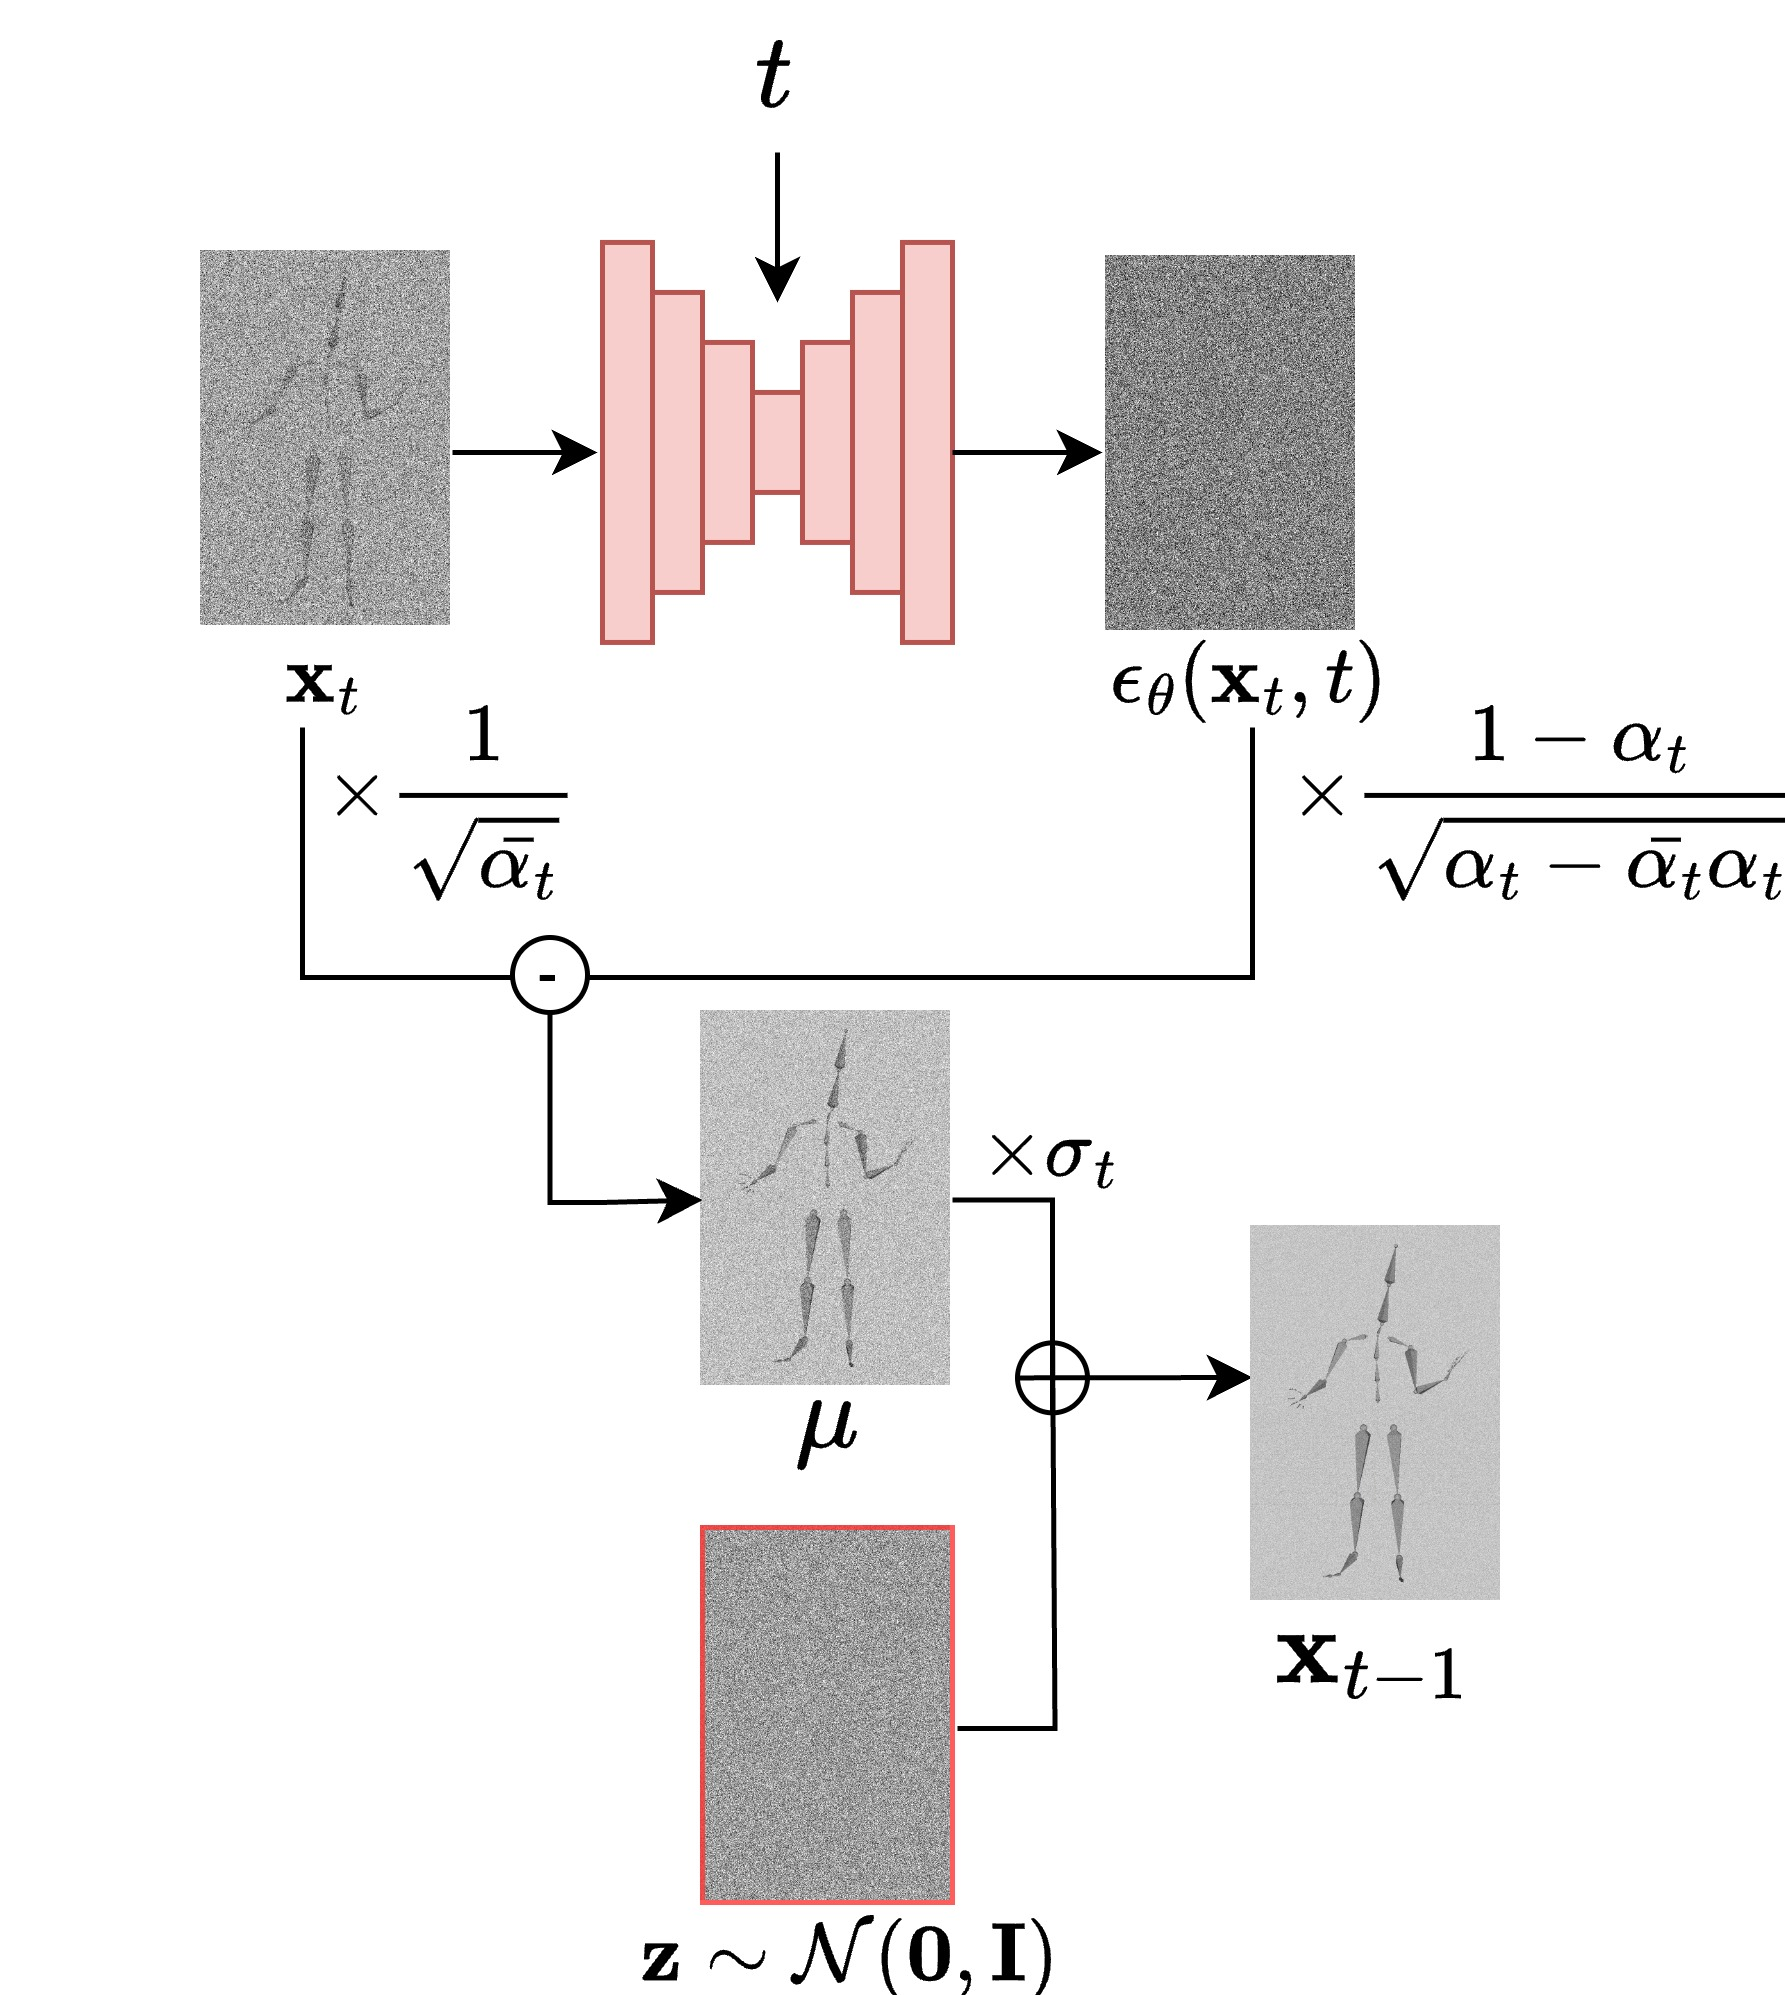
\includegraphics[height=280pt]{AlgorithmSamplingDiffusion}
	\caption{Khử nhiễu trong quá trình suy luận}
	\label{fig:AlgorithmSamplingDiffusion}
	\vspace{-5pt}
\end{figure}

Quá trình khử nhiễu $p_\theta(\mathbf{x}_{t-1} \vert \mathbf{x}_t)$  ở bước thứ $t$ từ $T \to 1$ được bắt đầu từ $\bx_T$ là nhiễu hoàn toàn $\mathcal{N} (\mathbf{0}, \mathbf{I})$. Luận văn sẽ dùng một neural network $f_{\theta} (\bx_t, t)$ để dự đoán nhiễu $\hat{\epsilon}_t = f_{\theta}(\bx_t, t)$ đã được thêm vào để được $\bx_{t-1}$ từ $\bx_t$.

Quá trình khử nhiễu có trung bình $\boldsymbol{\mu}_\theta(\mathbf{x}_t, t) = {\frac{1}{\sqrt{\alpha_t}} \Big( \mathbf{x}_t - \frac{1 - \alpha_t}{\sqrt{1 - \bar{\alpha}_t}}  f_\theta(\mathbf{x}_t, t) \Big)}$ và phương sai $\boldsymbol{\Sigma}_\theta(\mathbf{x}_t, t)$ như sau:

\begin{equation}
	\label{eq:denoising_process}
	\begin{aligned}
		p_\theta(\mathbf{x}_{0:T})
		&= p(\mathbf{x}_T) \prod^T_{t=1} p_\theta(\mathbf{x}_{t-1} \vert \mathbf{x}_t) \\
		p_\theta(\mathbf{x}_{t-1} \vert \mathbf{x}_t) &= \mathcal{N}(\mathbf{x}_{t-1};  \boldsymbol{\mu}_\theta(\mathbf{x}_t, t), \boldsymbol{\Sigma}_\theta(\mathbf{x}_t, t))
	\end{aligned}
\end{equation}

Quá trình khử nhiễu là quá trình bắt đầu từ nhiễu hoàn toàn, dùng một neural network $f_\theta$ để học được quá trình khử nhiễu.


\subsection{Quá trình huấn luyện trong mô hình diffusion cơ bản}
%	Hàm mất mát $\mathcal{L}$ của mô hình diffusion
	
	\begin{figure}[H]
		\centering
		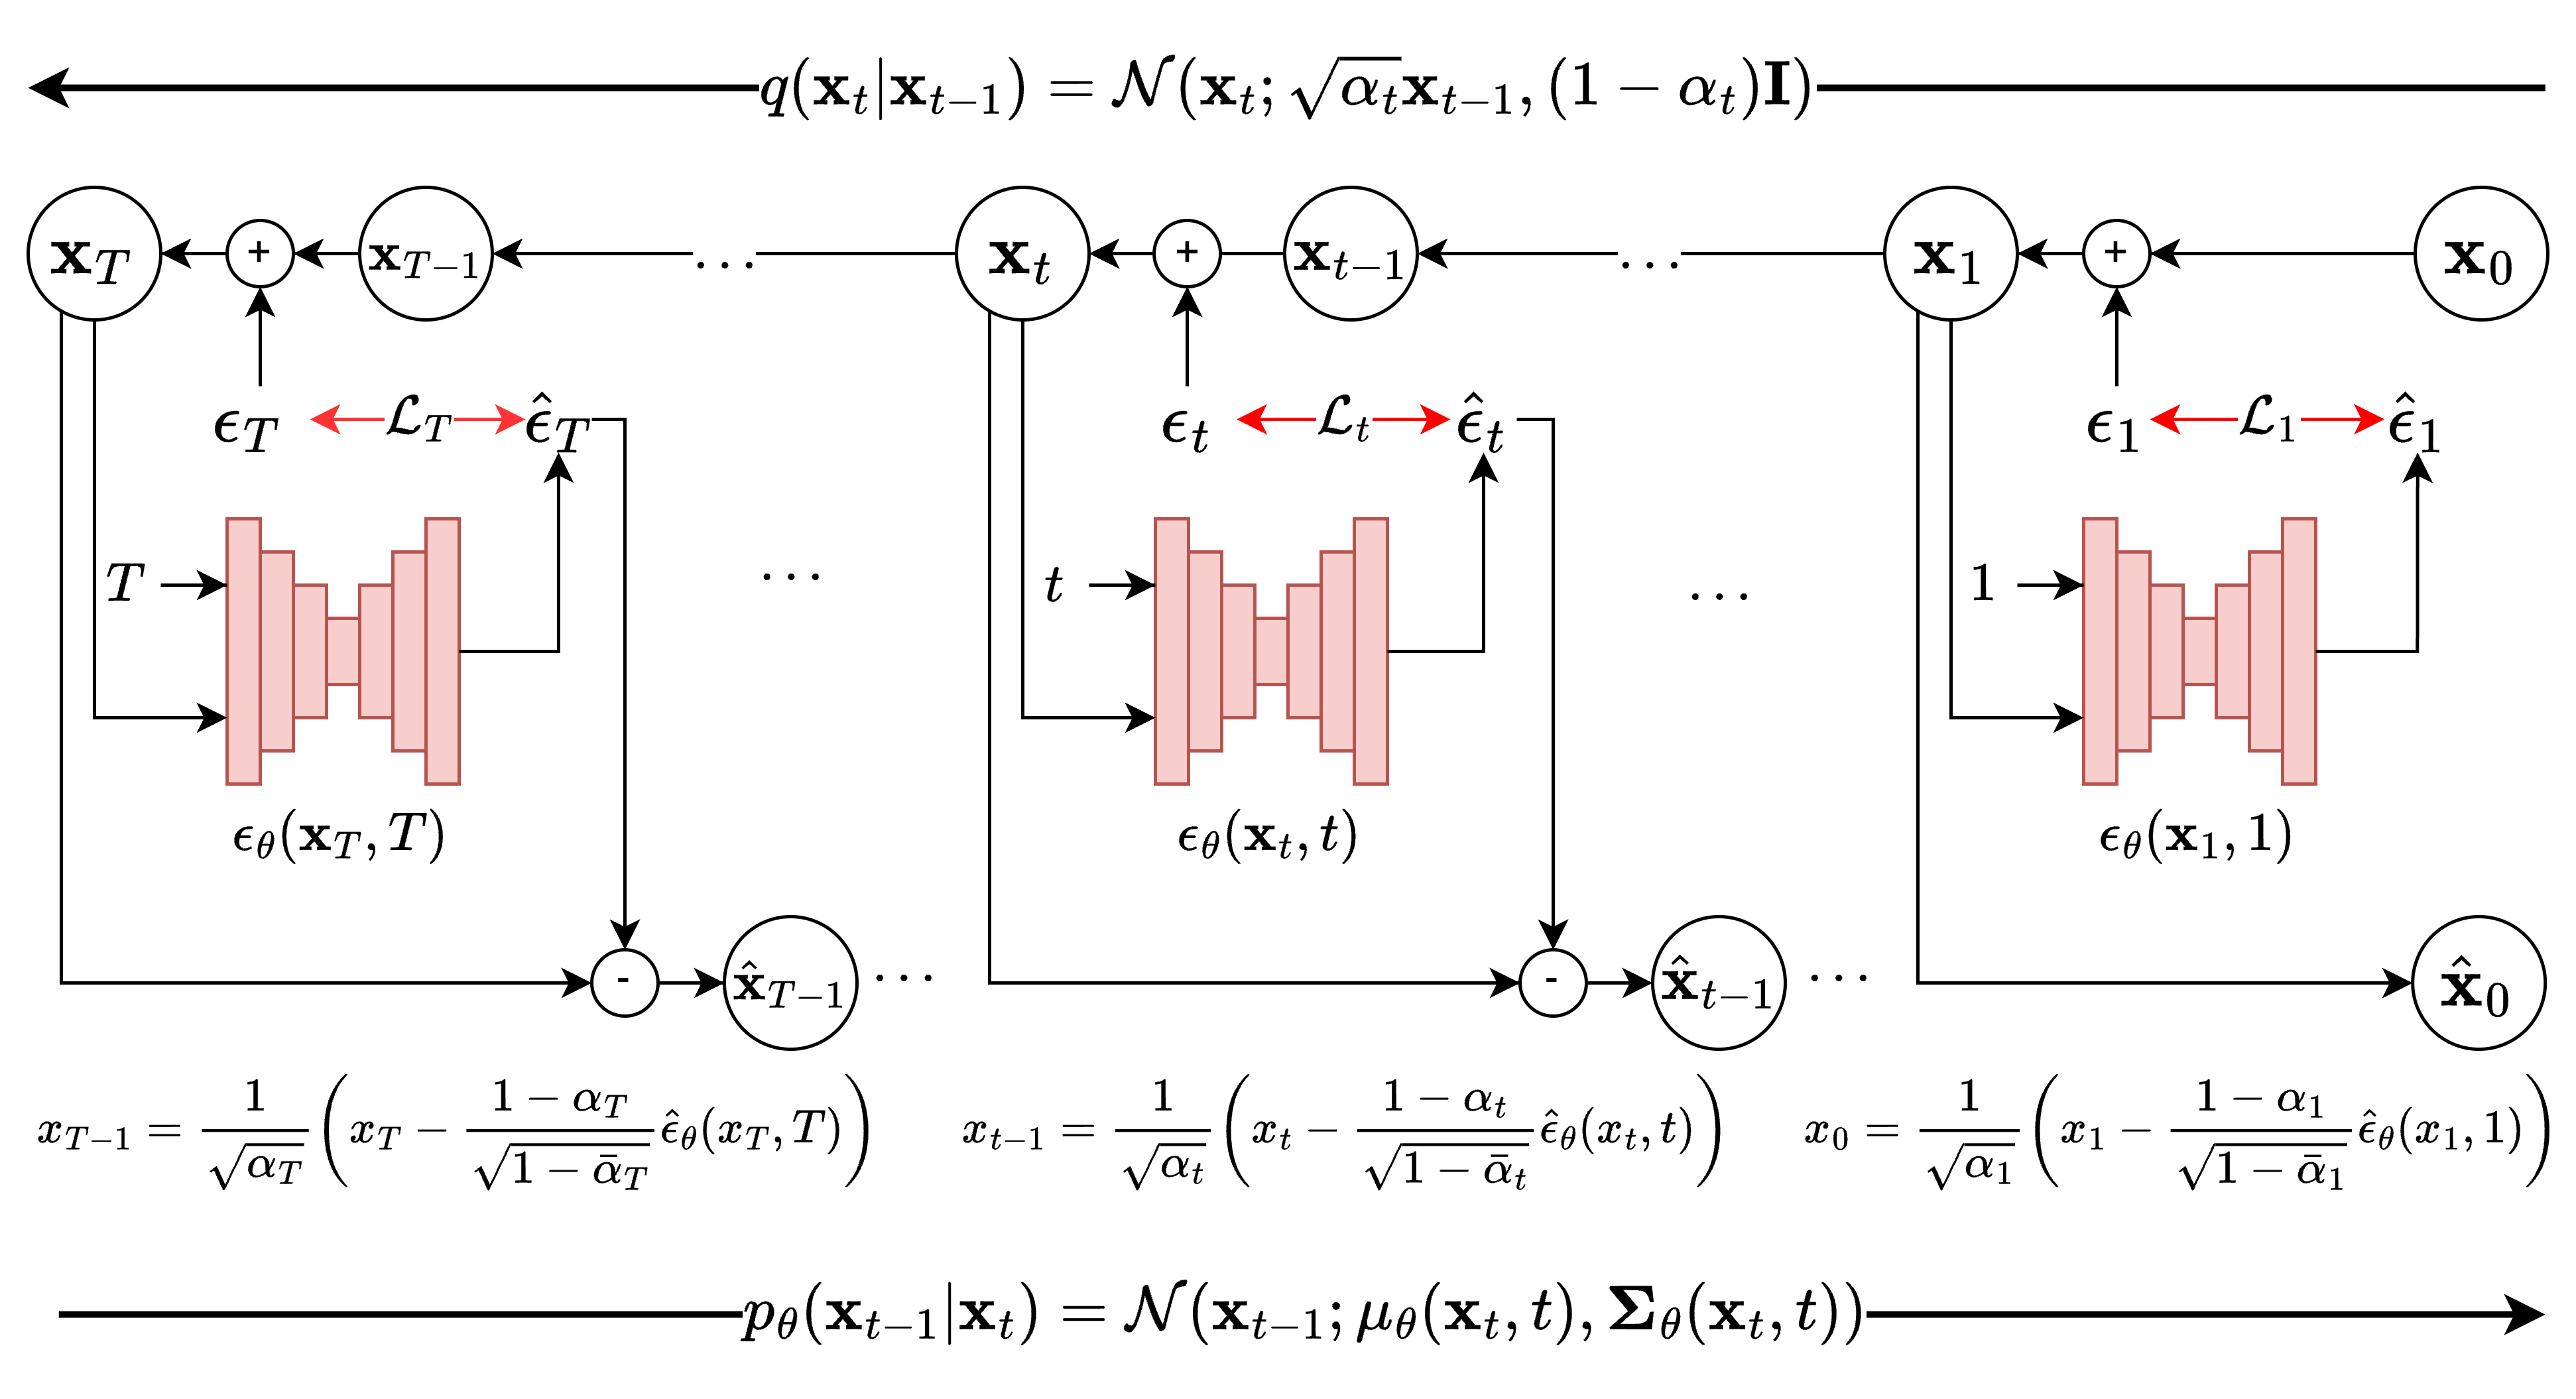
\includegraphics[width=\linewidth]{DDPMTraining}
		\caption{Mô hình diffusion cơ bản}
		\label{fig:basic_diffusion}\
		\vspace{-5pt}
	\end{figure}
	
	Mô hình diffusion sẽ học trọng số $\theta$ của hàm dự đoán lỗi $f_{\theta} (x_t, t)$ hay còn ký hiệu là  $\epsilon_{\theta} (x_t, t)$. Trong quá trình denoising, ta sẽ tối ưu độ lỗi giữa nhiễu dự đoán $\boldsymbol{\epsilon}_\theta(\mathbf{x}_t, t)$ và nhiễu thực tế $\boldsymbol{\epsilon}_t$. Với mỗi bước thứ $t$ ta sẽ tối ưu hàm loss $\mathcal{L}_{t}$ để thu được trọng số $\theta$.
	
	\begin{equation}
		\label{eq:diffusion_loss}
		\begin{aligned}
			\mathcal{L}^t
			&= \mathbb{E}_{t \sim [1, T], \mathbf{x}_0, \boldsymbol{\epsilon}_t} \Big[\|\boldsymbol{\epsilon}_t - \boldsymbol{\epsilon}_\theta(\mathbf{x}_t, t)\|^2 \Big] \\
			&= \mathbb{E}_{t \sim [1, T], \mathbf{x}_0, \boldsymbol{\epsilon}_t} \Big[\|\boldsymbol{\epsilon}_t - \boldsymbol{\epsilon}_\theta(\sqrt{\bar{\alpha}_t}\mathbf{x}_0 + \sqrt{1 - \bar{\alpha}_t}\boldsymbol{\epsilon}_t, t)\|^2 \Big]
		\end{aligned}
	\end{equation}


Trong đó, hàm mất mát $\mathcal{L}$ tổng sẽ là  $\mathcal{L} = \sum_{t=1}^{T} \mathcal{L}^t$.

Với $f_{\theta}(x_{t-1}, t)$ hay $\epsilon_\theta$ là một mô hình Unet dùng để mã hóa và giải mã dữ liệu để dự đoán nhiễu đã thêm vào dữ liệu. Quá trình tính toán hàm lỗi được trình bày minh họa trong \autoref{fig:basic_diffusion}.


\begin{algorithm}[H]
	
	\setlength{\baselineskip}{10pt}
	\begin{enumerate}
		\vspace{5pt}
		\item Tính sẵn các giá trị $\sqrt{\alpha_t}$, $\sqrt{1 - \alpha_t}$ và $\sqrt{\bar{\alpha}_t}$ cho mỗi bước $t: 1 \rightarrow T$. Xác định lịch trình nhiễu $\{\alpha_t \in (0, 1)\}_{t=1}^T$, với $\alpha_1 < \alpha_2 < \dots < \alpha_T$.
		
		\item Lấy nhãn $\mathbf{x}_0$ từ phân phối của dữ liệu đã chuẩn hóa.
		
		\item Tạo nhiễu ngẫu nhiên $\boldsymbol{\epsilon}_t$ cho mỗi bước $t: 1 \rightarrow T$, với $\forall t: \boldsymbol{\epsilon}_t \sim \mathcal{N}(\mathbf{0}, \mathbf{I})$.
		
		\item Gây nhiễu (forward) $\mathbf{x}_0$ để thu được $\mathbf{x}_t$ ở mỗi bước $t: 1 \rightarrow T$:
		$$
		\mathbf{x}_t = \sqrt{\bar{\alpha}_t} \mathbf{x}_0 + \sqrt{1 - \bar{\alpha}_t} \boldsymbol{\epsilon}_t
		$$
		
		\item Với mỗi $t$, lấy $t$ \textbf{ngẫu nhiên} từ $[1, T]$.
		
		\item Cho $\mathbf{x}_t$ và $t$ vào mô hình để dự đoán nhiễu: $\hat{\boldsymbol{\epsilon}} = \boldsymbol{\epsilon}_\theta(\mathbf{x}_t, t)$.
		
		\item Tính đạo hàm để cập nhật trọng số:
		$$
		\grad_{\theta_t} \left\| \boldsymbol{\epsilon}_t - \boldsymbol{\epsilon}_\theta(\mathbf{x}_t, t) \right\|^2
		$$
		
		Tính loss:
		$$
		\mathcal{L}^t = \mathbb{E}_{t \sim [1, T], \mathbf{x}_0, \boldsymbol{\epsilon}_t} \left[ \|\boldsymbol{\epsilon}_t - \boldsymbol{\epsilon}_\theta(\sqrt{\bar{\alpha}_t} \mathbf{x}_0 + \sqrt{1 - \bar{\alpha}_t} \boldsymbol{\epsilon}_t, t)\|^2 \right]
		$$
		
		\item Quay lại bước 6 cho đến khi hội tụ để thu được trọng số tối ưu $\theta'$.
	\end{enumerate}
	\caption{Thuật toán training trong DDPM}
	\label{alg:TrainingDDPM}
\end{algorithm}


\subsection{Quá trình lấy mẫu trong diffusion cơ bản}
	
		\begin{figure*}
		\centering
		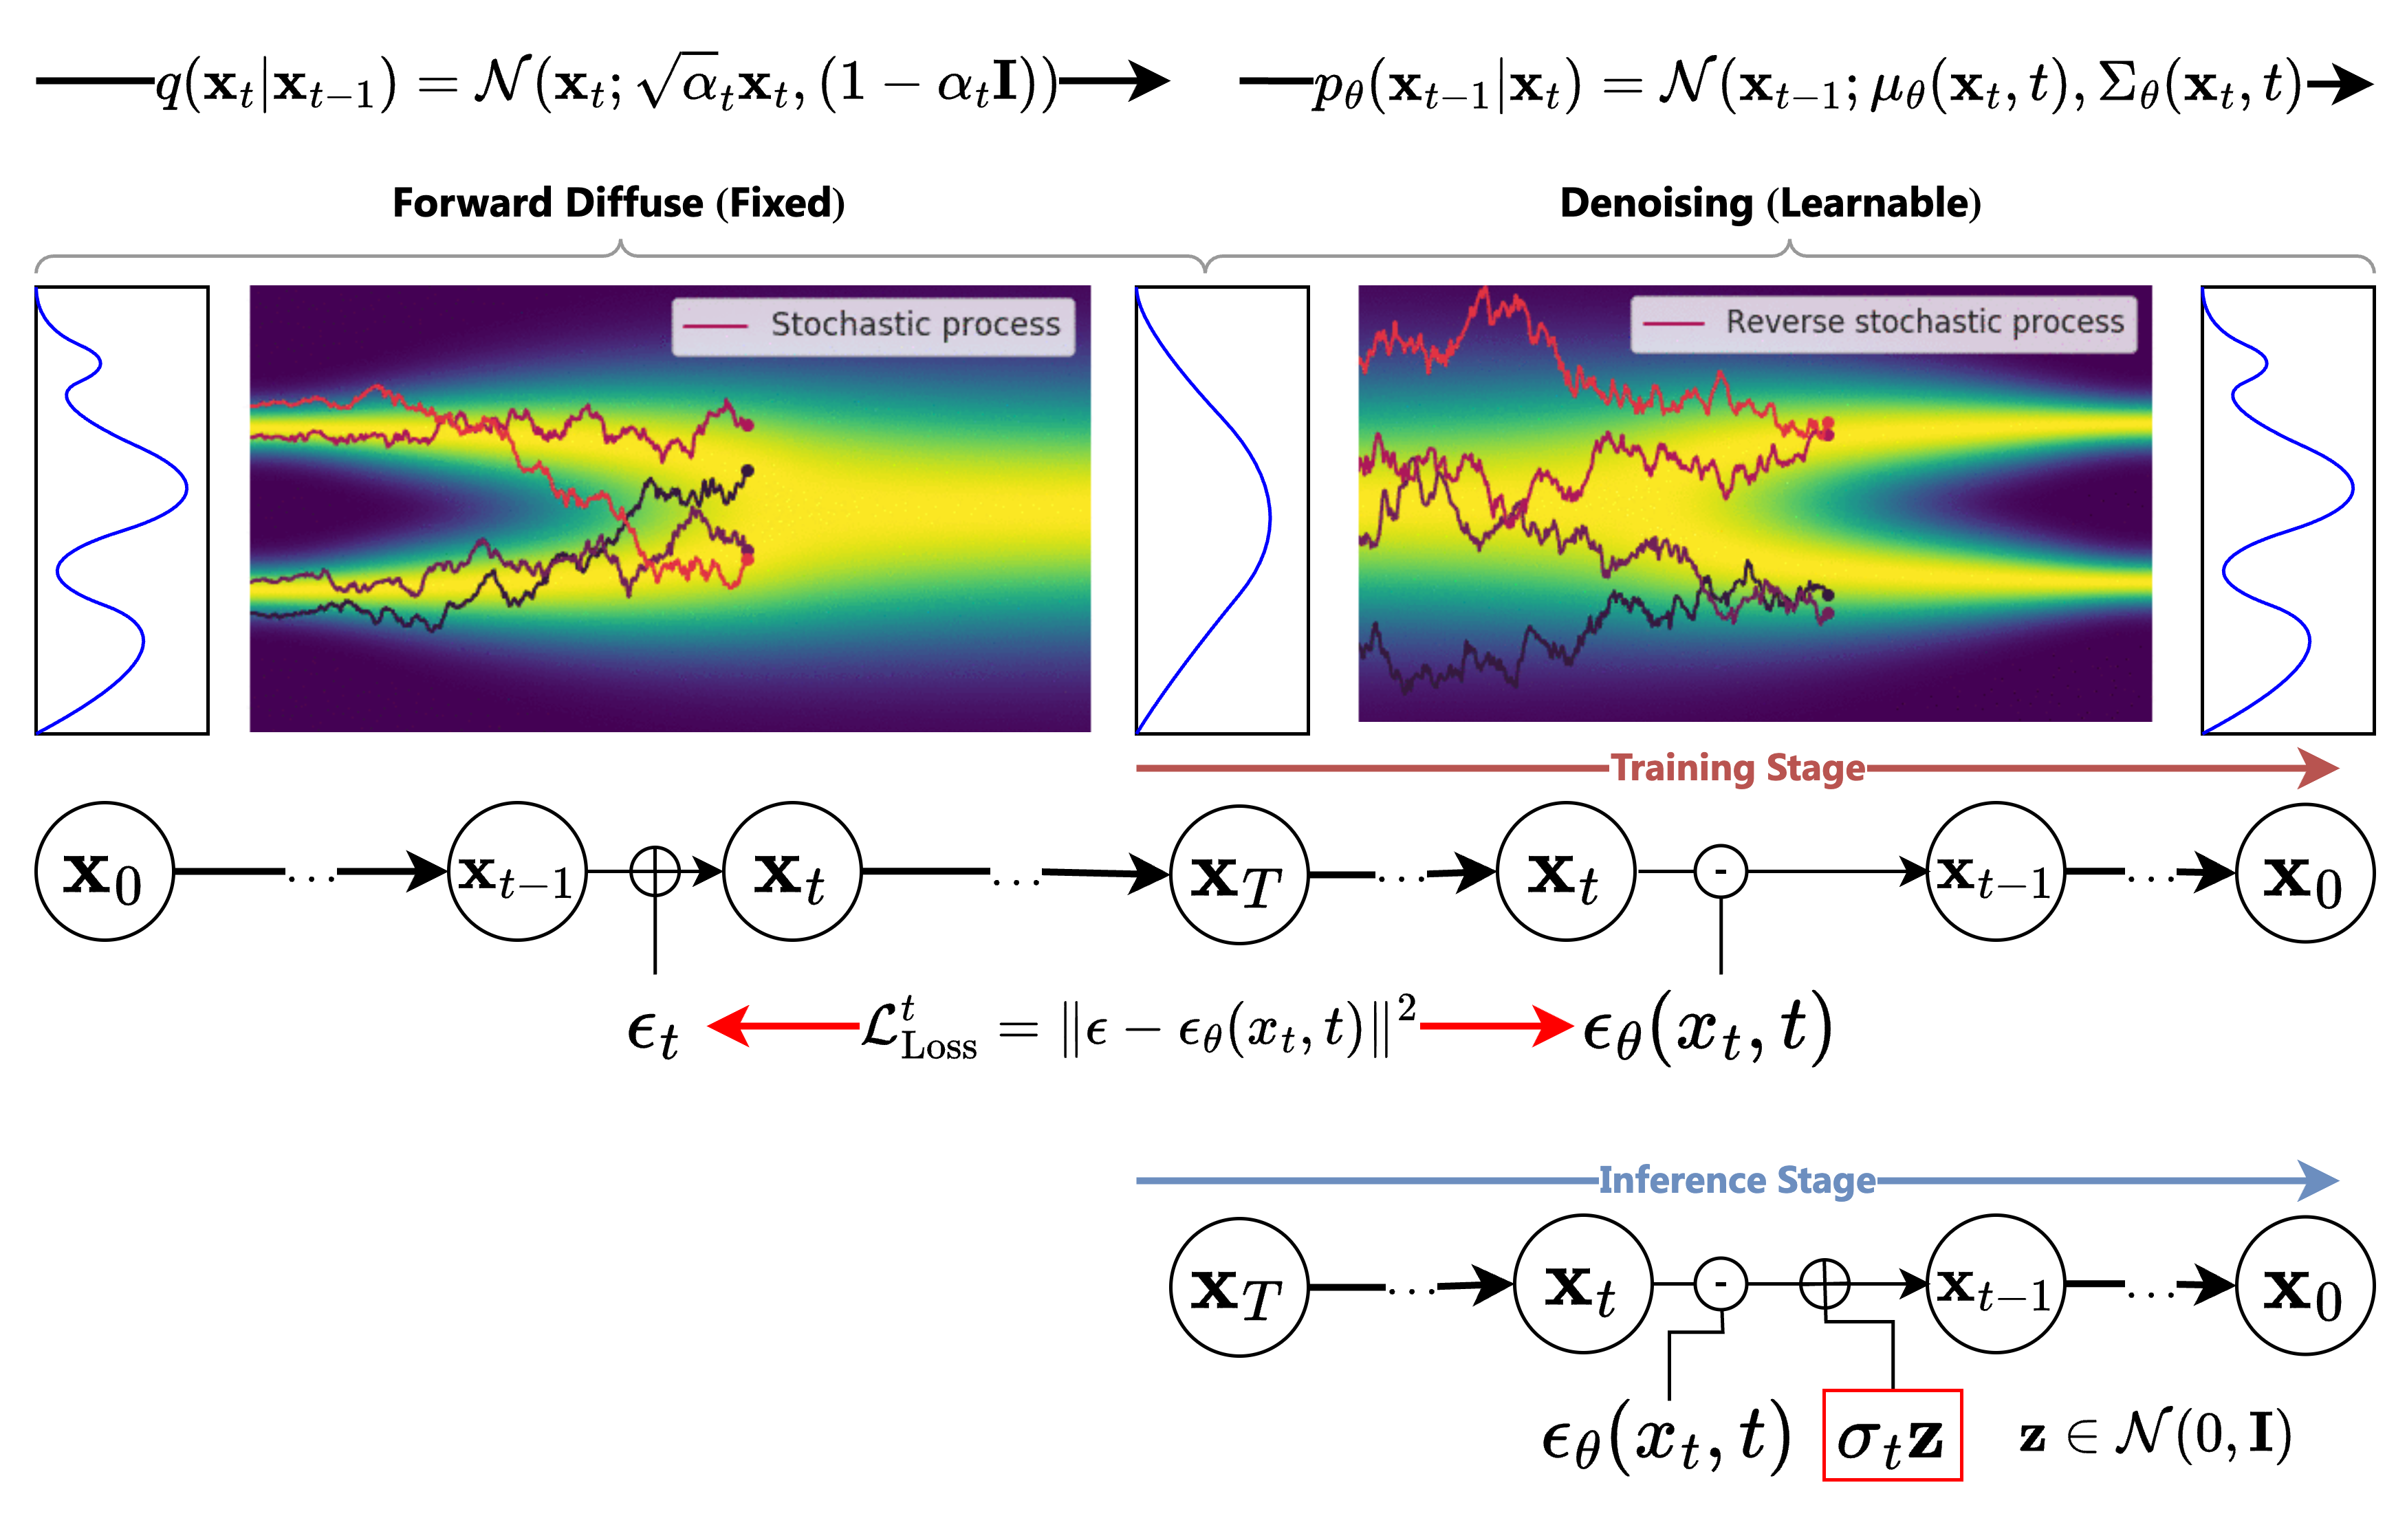
\includegraphics[width=\linewidth]{TrainingAndSamplingStandard}
		\caption{Quá trình Training và Sampling trong mô hình Diffusion tiêu chuẩn}
		\label{fig:GaussianDrift}
	\end{figure*}
	

	Sau khi thu được trọng số $\theta'$, luận văn sẽ dùng hàm denoising để khử nhiễu từ nhiễu $\bx_T \sim \mathcal{N} (\mathbf{0}, \mathbf{I})$.
	Quá trình biến đổi từ nhiễu hoàn toàn $\bx_{T}$ sang dự đoán $\hat{\bx_0}$ như sau:
	%với $t$ là một vector đã được nhúng vị trí bằng thuật toán nhúng
	
	\begin{equation}
		\label{eq:adddenoising}
	\bx_{t-1} = \frac{1}{\sqrt{\alpha_t}} \left( \bx_t - \frac{1- \alpha_t}{\sqrt{1 - \bar{\alpha}_t}} f_{\theta'}(\bx_t, t) \right) + \sqrt{1 - \alpha_t} \tilde{\epsilon}_t
	\end{equation}
	
Lưu ý rằng $\epsilon_t$ là nhiễu cố định và nhiễu ngẫu nhiên được tạo ra trước quá trình huấn luyện, chỉ sử dụng lại kết quả ngẫu nhiên trong quá trình forward diffusion \autoref{subsection:denoising_process} ở công thức  \autoref{eq:addgaussian}. Như \autoref{fig:GaussianDrift}, độ lỗi $\epsilon_t$ là độ nhiễu của từng bước $t$, và hàm loss  $\mathcal{L}^{t}$ sẽ tính theo từng bước $t$.


Tiếp theo quá trình huấn luyện, thuật toán lấy mẫu (sampling) trong DDPM bắt đầu từ bước tạo nhiễu hoàn toàn, tức là $\mathbf{x}_T \sim \mathcal{N}(0, \mathbf{I})$, nơi dữ liệu ban đầu hoàn toàn là nhiễu. Các giá trị $\sqrt{\alpha_t}$, $\sqrt{1 - \alpha_t}$ và $\sqrt{\bar{\alpha}_t}$, được tính từ quá trình huấn luyện, sẽ được sử dụng trong quá trình lấy mẫu để dự đoán lại dữ liệu gốc $\mathbf{x}_0$. Bước tiếp theo là tính toán hệ số điều chỉnh nhiễu $\sigma_t$, dựa vào lịch trình nhiễu $\alpha_t$ đã được thiết lập trong quá trình huấn luyện. Các giá trị này sẽ ảnh hưởng đến độ nhiễu được thêm vào trong quá trình lấy mẫu ngược.

Quá trình lấy mẫu (sampling) như \autoref{alg:samplingddpm} sẽ được thực hiện từ bước $T$ trở về $1$, và trong mỗi bước, một nhiễu ngẫu nhiên $\mathbf{z} \sim \mathcal{N}(0, \mathbf{I})$ được tạo ra để cộng thêm vào kết quả dự đoán. Tại mỗi bước $t$, mô hình sẽ dự đoán nhiễu $\boldsymbol{\epsilon}_{\theta'}$ dựa trên dữ liệu nhiễu $\mathbf{x}_t$ và bước thời gian $t$, sau đó sử dụng dự đoán này để tính toán giá trị $\mu$, là ước lượng của $\mathbf{x}_0$. Cuối cùng, một lượng nhiễu $\sigma_t \mathbf{z}$ được cộng thêm vào $\mu$ để thu được $\hat{\mathbf{x}}_{t-1}$, dữ liệu nhiễu tại bước $t-1$. Quá trình này tiếp tục cho đến khi $t = 1$, và khi đó, chúng ta có được $\hat{\mathbf{x}}_0$ — dự đoán cuối cùng của dữ liệu gốc từ quá trình khử nhiễu.

\begin{algorithm}[H]
	\caption{Thuật toán sampling trong DDPM}
	\label{alg:samplingddpm}
	\setlength{\baselineskip}{10pt}
	\begin{enumerate}
		\item Bắt đầu với nhiễu: $\mathbf{x}_T \sim \mathcal{N}(0, \mathbf{I})$.
		
		\item Các giá trị $\sqrt{\alpha_t}$, $\sqrt{1 - \alpha_t}$ và $\sqrt{\bar{\alpha}_t}$ được lấy từ quá trình huấn luyện.
		
		\item Tính hệ số điều chỉnh nhiễu $\sigma_t$ từ $\alpha_t$ ở mỗi bước $t: 1 \rightarrow T$:
		\[
		\sigma_t = \sqrt{\frac{1 - \bar{\alpha}_{t-1}}{1 - \bar{\alpha}_t} (1 - \alpha_t)}
		\]
		
		\item Với mỗi $t$, lấy $t$ \textbf{tuần tự} từ $[T, \dots, 1]$.
		
		\item Tạo nhiễu ngẫu nhiên $\mathbf{z} \sim \mathcal{N}(0, \mathbf{I})$.
		
		\item Đưa $\mathbf{x}_t$ vào mô hình để suy luận nhiễu: $\boldsymbol{\epsilon}_{\theta'} = \boldsymbol{\epsilon}_{\theta'}(\mathbf{x}_t, t)$.
		
		\item Dùng nhiễu dự đoán để trừ đi $\mathbf{x}_t$ ở bước $t$:
		\[
		\mu = \frac{1}{\sqrt{\alpha_t}} \left( \mathbf{x}_t - \frac{1 - \alpha_t}{\sqrt{1 - \bar{\alpha}_t}} \boldsymbol{\epsilon}_{\theta'}(\mathbf{x}_t, t) \right)
		\]
		
		\item Cộng thêm một lượng nhiễu: $\hat{\mathbf{x}}_{t-1} = \mu + \sigma_t \mathbf{z}$.
		
		\item Khi $t = 1$, thu được $\hat{\mathbf{x}}_0$ từ quá trình khử nhiễu.
	\end{enumerate}

\end{algorithm}

Điều quan trọng nhất trong quá trình lấy mẫu (denoising sampling) đó chính là phải cộng thêm một độ nhiễu $\mathbf{z} \in \mathcal{N}(0, \mathbf{I})$, với $\mathbf{z}$  sẽ được lần lượt thêm ở từng bước $t$ bằng hệ số điều khiển $\sigma_t$. Mục tiêu của nhiễu $\epsilon$ là để  làm gờ phân phối (marginal noise distribution) cho mô hình $f_\theta$ (hay $\epsilon_{\theta}$) có thể học được nhiễu, còn với  $\mathbf{z}$ là để tăng tính đa dạng trong quá trình sinh và sự ổn định trong quá trình lấy mẫu. Quá trình giảm $\sigma_t$ được trình bày ở phụ lục \autoref{appendix:Appendix1:NoiseScale}


\subsection{Cải tiến mô hình diffusion với dự đoán $\bx_0$ thay vì $\epsilon_t$}
\label{subsec:X0Objective}

Dựa vào \autoref{eq:tracexzero}, có thể thấy nếu có $\bx_{t}$ thì sẽ suy ra được $\bx_0$. Và nếu có $\bx_0$ thì cũng sẽ có thể suy ra được $\bx_{t}$ \textbf{một cách tường minh} với $t$ bất kỳ bằng cách thêm nhiễu $\epsilon_t$ đã có từ quá trình thêm nhiễu thuận (forward diffusion).

Từ quan sát này, nhóm tác giả \cite{nichol2021improved} đề xuất cải tiến DDPM, thay vì dùng hàm neural network $f_{\theta}(\bx_t, t)$ để dự đoán $\epsilon_t$ như \autoref{fig:basic_diffusion} thì $f_{\theta}(\bx_t, t)$ sẽ được dùng để dự đoán trực tiếp $\bx_0$, và khi có $\bx_0$ sẽ thêm nhiễu bằng  \autoref{eq:tracexzero}


\begin{figure}[H]
	\captionsetup{skip=2pt}
	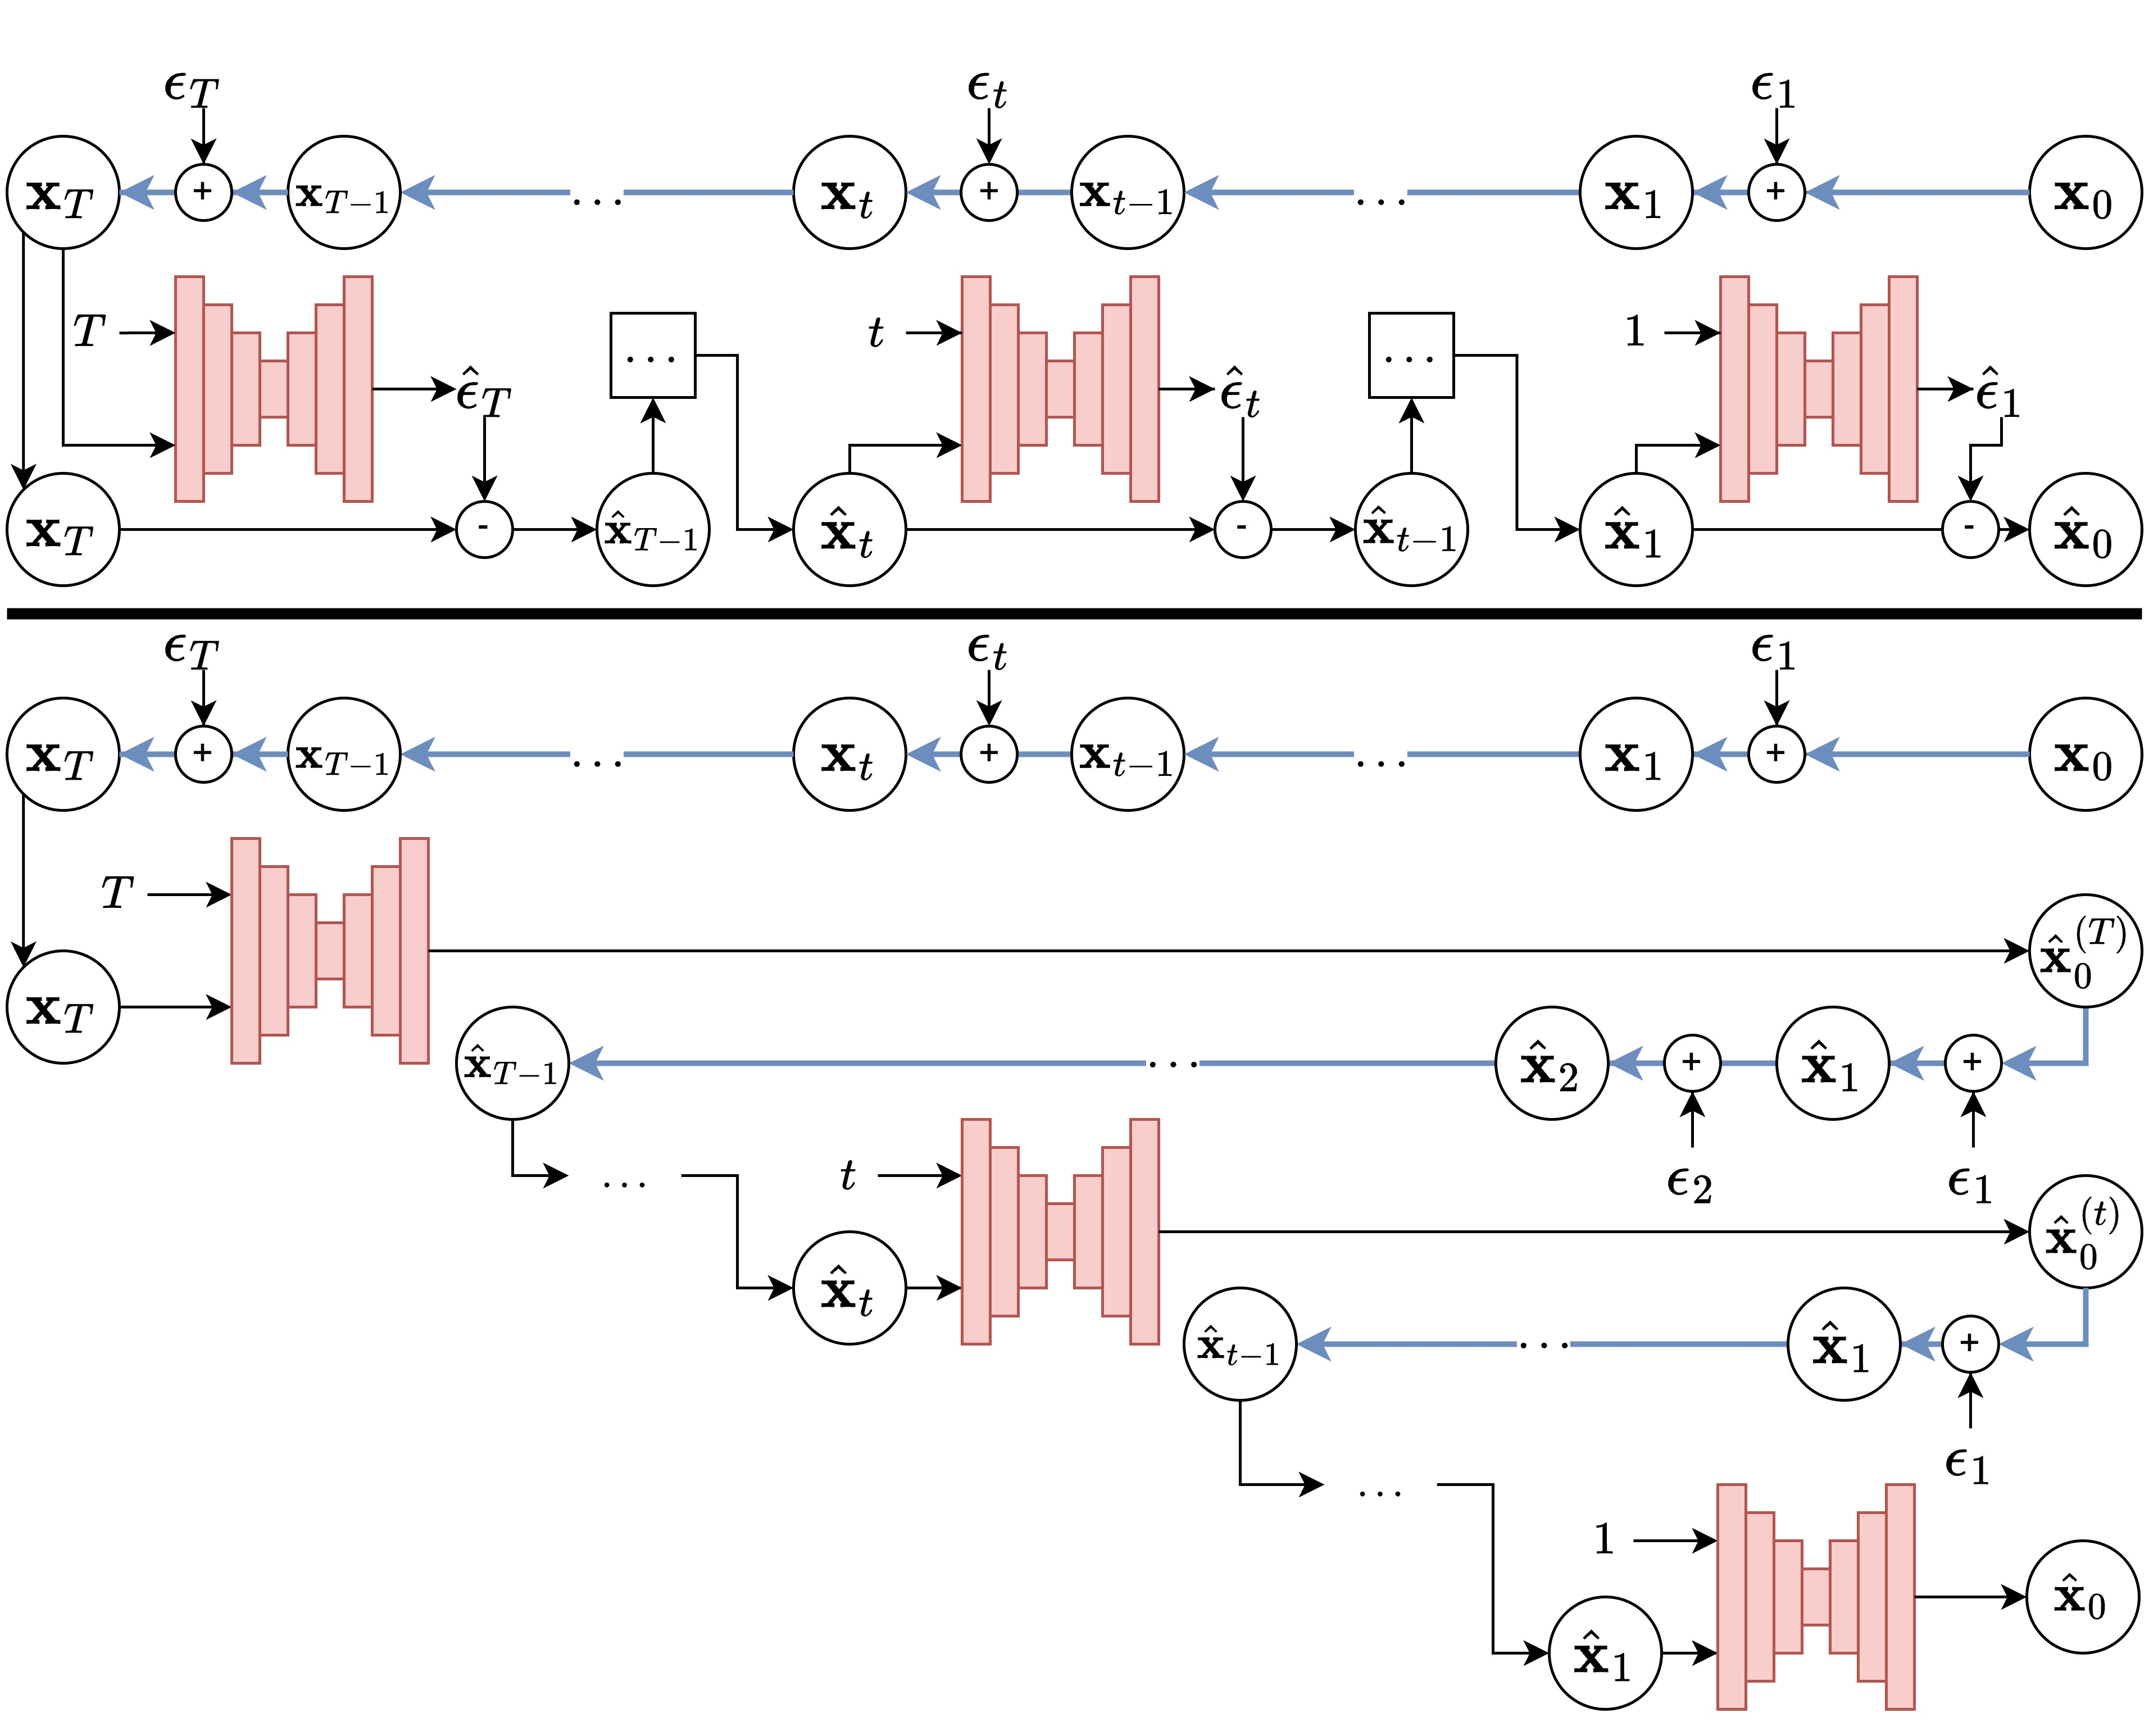
\includegraphics[width=\linewidth]{X0Objective}
	\caption{So sánh $\epsilon$ objective (bên trên) và  $\bx_0$ objective (bên dưới)}
	\label{fig:X0Objective}
\end{figure}

Như hình \autoref{fig:X0Objective}, ta bắt đầu bằng việc thêm nhiễu thuận (forward diffusion), từ $t: 1 \rightarrow T$ để được $\bx_T \sim \mathcal{N} (0, \mathbf{I})$. Sau khi có nhiễu $\bx_{T}$ ta sẽ đưa vào hàm $f_{\theta}$ để dự đoán $\hat{\bx}_0$, từ $\hat{\bx}_0$ sẽ thêm nhiễu để được $\hat{\bx}_{t-1}$. Thực hiện lần lượt đến khi $t = 1$, ta sẽ thu được $\hat{\bx}_0$. Ta có thể so sánh hai phương pháp như sau:

\begin{itemize}
	\item \textbf{$\epsilon$  objective} :  mô hình sẽ dự đoán lỗi. Bắt đầu từ việc forward quá trình gây nhiễu để lấy được $\bx_T$, khi có được $\bx_T$ ta sẽ sử dụng $\bx_T \in \mathcal{N}(0, \mathbf{I})$ để đưa vào quá trình denoise. Trong quá trình khử nhiễu, mô hình sẽ dự đoán nhiễu $\hat{\epsilon}_t$ đã được thêm vào từ quá trình forward, là nhiễu $\epsilon_t$ và tối ưu lỗi giữa nhiễu dự đoán và nhiễu thực tế từ quá trình forward.
	\item \textbf{$\bx_0$ objective} : tương tự mô hình sẽ gây nhiễu (forward diffusion) quá trình gây nhiễu để lấy được $\bx_T$, khi có được $\bx_T$ ta sẽ sử dụng $\bx_T \in \mathcal{N}(0, \mathbf{I})$ để đưa vào quá trình denoise. Mô hình sẽ dự đoán trực tiếp $\bx_0$, sau khi có $\bx_0$ mô hình sẽ tiếp tục gây nhiễu đến bước thứ $\bx_{t-1}$, và tiếp tục sử dụng $\bx_{t-1}$ để đưa vào mô hình dự đoán $\bx_0$
\end{itemize}

\subsection{Mô hình diffusion có điều kiện}
\label{subsec:DiffusionCondition}

Để có thể điều khiển quá trình sinh với các điều kiện khác nhau, thì cần phải sinh với điều kiện $c$, hay nói cách khác ta cần tìm xác suất $p(\bx | c)$ khi biết trước $c$. Nhóm tác giả \cite{dhariwal2021diffusion} đề xuất sử dụng một hàm $f_{\phi}$ riêng để huấn luyện cho điều kiện. Tuy nhiên phương pháp này gây khó khăn khi các điều kiện sinh thay đổi và việc kết hợp và cập nhật trọng số ở một mô hình riêng sẽ gây khó khăn khi mở rộng.

\begin{figure}[H]
	\captionsetup{skip=20pt}
	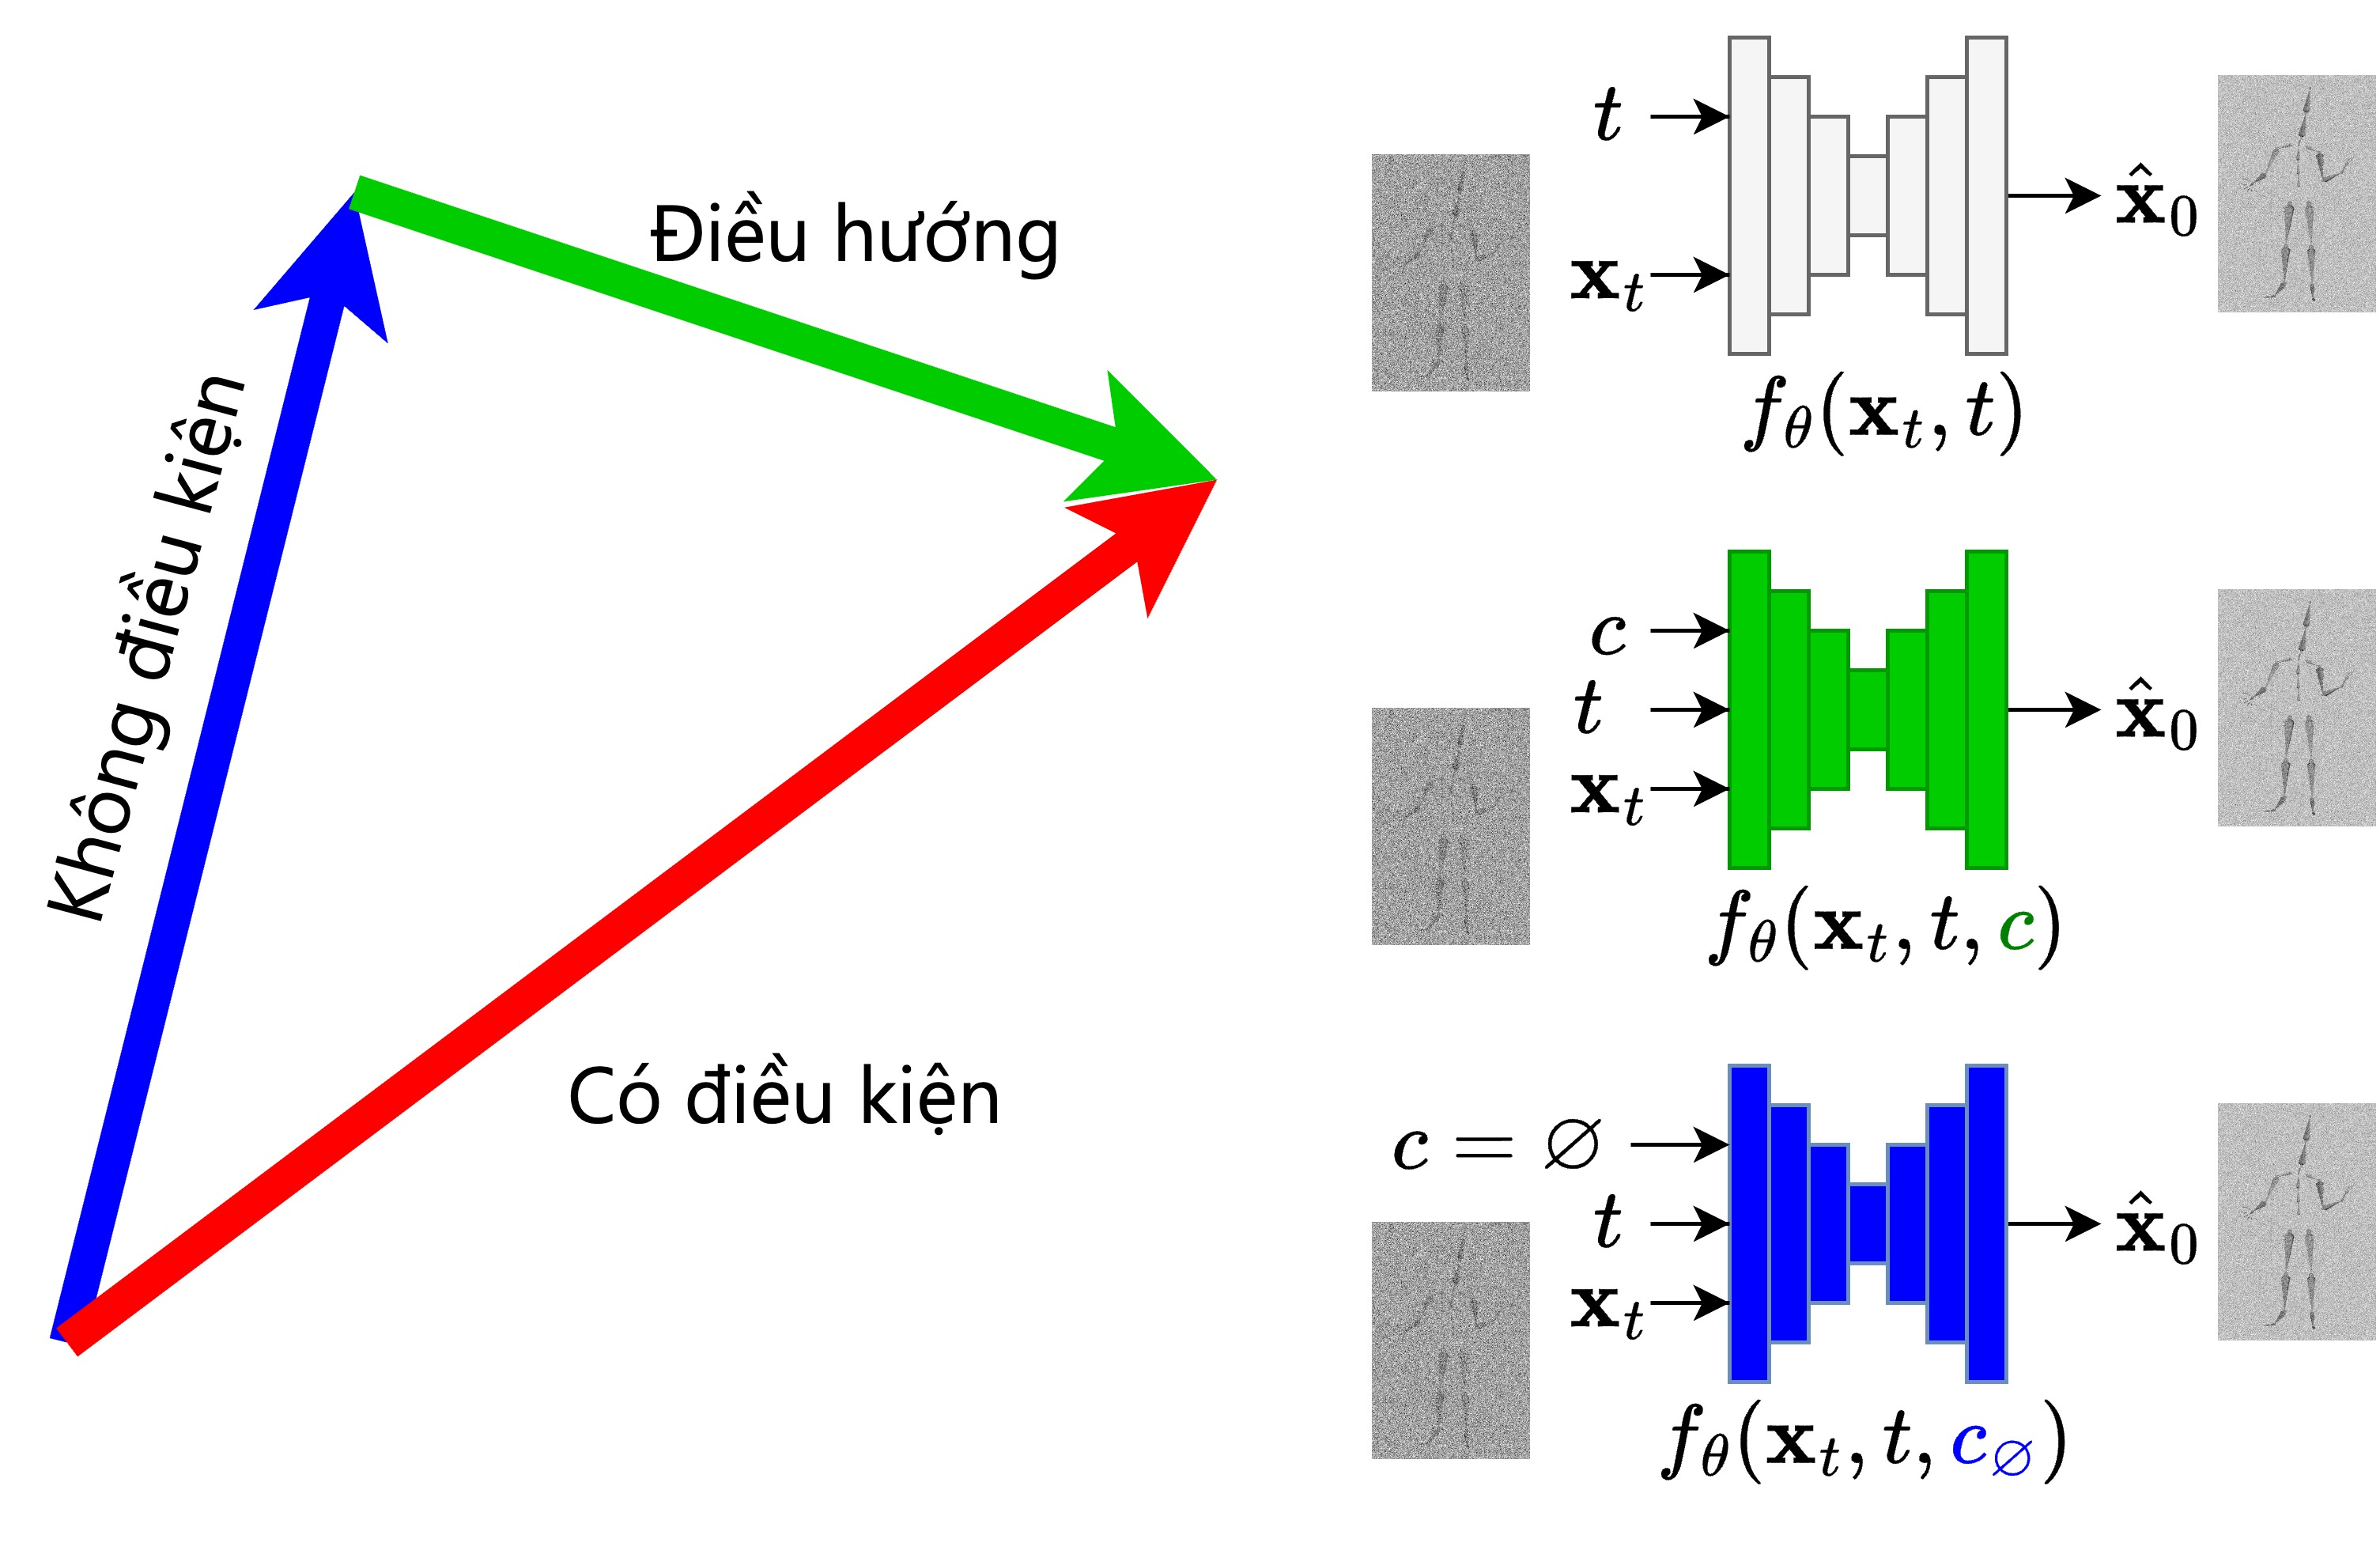
\includegraphics[width=0.9\linewidth]{AdversarialGradient}
	\caption{Diffusion có điều kiện bằng vector điều hướng}
	\label{fig:AdversarialGradient}
\end{figure}

Như hình \autoref{fig:GaussianDrift}, để quá trình suy luận có thể sinh ra các kết quả $\bx_0$ khác nhau và có thể điều khiển được dựa trên điều kiện $c$. Ở mỗi bước $t$, cần thêm một lượng điều hướng với một điều kiện cụ thể. Nhóm tác giả đề xuất  Classifier-Free Diffusion Guidance \cite{ho2022classifier} với việc kết quả $\bx_0$ được cập nhật bằng cách cộng kết quả có điều kiện và không có điều kiện.
\begin{equation}
{\color{red}{\hat{\mathbf{x}}}}_{0 \gamma, \color{blue}{c}, \color{green}{c_{\varnothing}}}=\gamma \cdot f_{\theta} \left(\mathbf{x}_{t}, t, {\color{blue}{c}} \right)+(1-\gamma) \cdot f_{\theta} \left(\mathbf{x}_{t}, t, {\color{green}{c_{\varnothing}}} \right)
\end{equation}

Trong đó, $c$ là điều kiện, $c_{\varnothing}$ là điều kiện rỗng,  kết quả sinh điều kiện được điều khiển bằng tham số $\gamma$, nếu $\gamma$ càng lớn thì kết quả sinh ra càng sát với điều kiện $c$, ngược lại thì kết quả sẽ nghiêng về kết quả sinh không có điều kiện.


Như \autoref{fig:AdversarialGradient}, hàm $f_{ \theta}$ trên cùng là không có điều kiện, $f_{ \theta}$ giữa là diffusion có điều kiện, $f_{ \theta}$ (dưới cùng) là diffusion với điều kiện rỗng.